% !TeX document-id = {acd94374-0a5a-4c39-a15c-8f2e56f0151a}
\documentclass[12pt,a4paper, listof=entryprefix, bibliography=totocnumbered,toc=listofnumbered,lof=listofnumbered]{scrartcl}

% WICHTIG!!!
% Pseudokommentar um pdflatex zu erlauben andere Programme zu nutzen z.B. gnuplot
% !TeX TXS-program:compile = txs:///pdflatex/[--shell-escape] 

\usepackage[ngerman]{babel}
\usepackage[utf8]{inputenc}
\usepackage{amsmath}
\usepackage{nccmath}
\usepackage{amsfonts}
\usepackage{amssymb}
\usepackage{graphicx}
\usepackage{fancyhdr}
\usepackage{tabularx}
\usepackage{geometry}
\usepackage{setspace}
\usepackage[right]{eurosym}
\usepackage[printonlyused]{acronym}
\usepackage{subfig}
\usepackage{floatflt}
\usepackage[usenames,dvipsnames]{color}
\usepackage{colortbl}
\usepackage{xcolor}
\usepackage{paralist}
\usepackage{array}
\usepackage{titlesec}
\usepackage{parskip}
\usepackage{picinpar}
\usepackage[pdfpagelabels=true]{hyperref}
\usepackage{listings}
\usepackage{csquotes}
\usepackage{url}
\usepackage{float}
\usepackage{pgfplots}
\usepackage{paralist}
\usepackage[nonumberlist, nogroupskip]{glossaries}

%-----------------------------------------------------------------------------------
% Bibilothek
%-----------------------------------------------------------------------------------
% Einbinden des BibLateX paketes mit Ausgabeeinstellungen
\usepackage[
style=alphabetic,          % Zitierstil
maxbibnames=50,            % alle Autorennamen anzeigen
maxcitenames=4,            % maximale Namen, die im Kürzel angezeigt werden
autocite=inline,           % regelt Aussehen für \autocite (inline=\parancite)
block=space,               % kleiner horizontaler Platz zwischen den Feldern
backref=true,              % Seiten anzeigen, auf denen die Referenz vorkommt
backrefstyle=three+,       % fasst Seiten zusammen, z.B. S. 2f, 6ff, 7-10
date=short,                % Datumsformat
backend = biber,           % Backnend für Aufbereitung
]{biblatex}

%Zusätzliche für Umbrüche für Kleinbuchstaben z.B. in URLs
\appto\UrlBreaks{\do\a\do\b\do\c\do\d\do\e\do\f\do\g\do\h\do\i\do\j
	\do\k\do\l\do\m\do\n\do\o\do\p\do\q\do\r\do\s\do\t\do\u\do\v\do\w
	\do\x\do\y\do\z}


\newcounter{verzeichnis}
\setcounter{verzeichnis}{1}

%Abstände der Einträge
\setlength{\bibitemsep}{1em}     % Abstand zwischen den Literaturangaben
\setlength{\bibhang}{2em}        % Einzug nach jeweils erster Zeile

% Kürzel soll vier Buchstaben der Autoren enthalten statt drei
\DeclareLabelalphaTemplate{
	\labelelement{
		\field[final]{shorthand}
		\field{label}
		\field[strwidth=4,strside=left,ifnames=1]{labelname}
		\field[strwidth=2,strside=left,ifnames=2]{labelname}
		\field[strwidth=1,strside=left]{labelname}
	}
	\labelelement{
		\field[strwidth=2,strside=right]{year}
	}
}

% Bibliothek der Quellen
\bibliography{bib}
\label{bib}

% --------------------------------------------------------------------------------
% Einstellung für Listings
% --------------------------------------------------------------------------------
\lstset{basicstyle=\footnotesize, captionpos=b, breaklines=true, showstringspaces=false, tabsize=2, frame=lines, numbers=left, numberstyle=\tiny, xleftmargin=2em, framexleftmargin=2em}
\makeatletter
\def\l@lstlisting#1#2{\@dottedtocline{1}{0em}{1em}{\hspace{1,5em} Lst. #1}{#2}}
\makeatother

% --------------------------------------------------------------------------------
% Seitenformate
% --------------------------------------------------------------------------------
%Seitenformat
\geometry{a4paper, top=27mm, left=30mm, right=20mm, bottom=32mm, headsep=12mm, footskip=12mm}

% --------------------------------------------------------------------------------
% Metainformationen
% --------------------------------------------------------------------------------
\hypersetup{unicode=false, pdftoolbar=true, pdfmenubar=true, pdffitwindow=false, pdfstartview={FitH},
	pdftitle={Vorlage},
	pdfauthor={Stefan Jung},
	pdfsubject={Abschlussarbeit},
	pdfcreator={\LaTeX\ with package \flqq hyperref\frqq},
	pdfproducer={pdfTeX \the\pdftexversion.\pdftexrevision},
	pdfkeywords={Vorlage},
	pdfnewwindow=true,
	colorlinks=true,linkcolor=black,citecolor=black,filecolor=magenta,urlcolor=black}
\pdfinfo{/CreationDate (D:20141024101000)}
\pgfplotsset{compat=1.11}

%-----------------------------------------------------------------------------------
% Abkürzungen AKRONYME HIER ERGÄNZEN
%-----------------------------------------------------------------------------------
\glssetwidest{HPPLAN}% Längste Abkürzung für eine korrekte Einrückung

\makenoidxglossaries %Leeres Verzeichnis erstellen

%Abkürzungen hinzufügen
\newacronym{LIP}{LIP}{Labor für Informationstechnik und Produktionslogistik}
\newacronym{JRE}{JRE}{Java Runtime Environment}
\newacronym{CLSP}{CLSP}{Capacitated Lot-Sizing Problem}
\newacronym{OTH}{OTHR}{Ostbayerische Technische Hochschule Regensburg}

\begin{document}
% --------------------------------------------------------------------------------
% Globale Formateinstellungen
% --------------------------------------------------------------------------------
\onehalfspacing
% Abstände Überschrift
\titlespacing{\section}{0pt}{42pt}{6pt}
\titlespacing{\subsection}{0pt}{12pt}{6pt}
\titlespacing{\subsubsection}{0pt}{12pt}{6pt}

% Kopf- und Fusszeile
\pagestyle{fancy}
\lhead{}\chead{}
\rhead{\thesection\space\contentsname}
\lhead{}\cfoot{}
\rfoot{\ \linebreak \thepage}
\renewcommand{\headrulewidth}{0.4pt}
\renewcommand{\footrulewidth}{0.4pt}

% Nummereriung
\renewcommand{\thesection}{\Roman{section}}
\renewcommand{\theHsection}{\Roman{section}}
\pagenumbering{Roman}

% eigene Farbdefinitionen
\definecolor{lip}{HTML}{3366FF}
\definecolor{grey}{HTML}{ABABAB}

% ---------------------------------------------------------------------------
% Titelseite
% ---------------------------------------------------------------------------
\thispagestyle{empty}

%LIP Schriftzug in eigener Farbe 
\textsf{\begin{minipage}{.69\textwidth}
	\large
	\textcolor{lip}{\textbf{Labor für Informationstechnik und\\Produktionslogistik (LIP)}} %Farbe setzten
	\small 
	\textbf{\\Verfahren, Strategien, Prozesse und IT-Systeme}
	\\Professor Dr.-Ing. Frank Herrmann
\end{minipage}
%Einbinden des OTH Logos mir rechtsbündiger Ausrichtung
\begin{minipage}{.29\textwidth}
	\begin{flushright}
		
\includegraphics[scale=.15]{images/othlogo}\\
	\end{flushright}
\end{minipage}}
 
% Zeilenabstand
\onehalfspacing	

%Beschriftung der Titelseite
\begin{center}

	\vspace*{4cm} %4 cm Vorspann
	\Large
	\textbf{Benutzerhandbuch zum Capacitated Lot-Sizing Problem}\\ %Titel der Arbeit
		
	\vspace*{8cm} %8 cm Vorspann
	\normalsize
	\begin{center}
	Aktueller Stand: \today 
	
	\textbf{Arnold Christiane \\ Butz Thomas \\ Denzin Timo \\ Eichinger Tobias \\ Gais Dominik \\ Liebich Johannes \\ Schertler Sascha \\ Sonnleitner Daniel \\ Wagner Pilar} %Name des Autors
	
	\end{center}
\end{center}
\pagebreak

% ------------------------------------------------------------------------------
% Inhaltsverzeichnis
% ------------------------------------------------------------------------------
% Inhaltsverzeichnis
\singlespacing %Zeilenabsatnd reduzieren
\setcounter{section}{0}
\setcounter{page}{1}
\addcontentsline{toc}{section}{Inhaltsverzeichnis}%hinzufügen des Inhaltsverzeichnises selbst

\tableofcontents %Ausgabe des Inhaltsverzeichnisses
\pagebreak

% ------------------------------------------------------------------------------
% Setzen der Nummerierungen für Normaltext
% ------------------------------------------------------------------------------
\onehalfspacing %Zeilenabstand auf 1.5
\renewcommand{\thesection}{\arabic{section}} %Arabische Beschriftung für Absatznummern
\pagenumbering{arabic}  %Seitennummerrierung auf arabisch setzten
\setcounter{page}{1}	%Seitenzahl für Inhalt auf 1 setzten
\setcounter{section}{0}
% Kopfzeile mit aktuellem Hauptkapitel darstellen
\renewcommand{\sectionmark}[1]{\markright{#1}} %Section ausgeben
\renewcommand{\subsectionmark}[1]{}            %Subsection nicht ausgeben
\renewcommand{\subsubsectionmark}[1]{}         %Subsubsection nicht ausgeben
\rhead{\rightmark}                             %Ausgabe Rechtsbündig

%------------------------------------------------------------------------------
%	Einfuehrung
%------------------------------------------------------------------------------
\section{Einführung}
\label{ch:einfuehrung}
Das vorliegende Dokument beschreibt die Handhabung und Funktionsweise der Software \gls{CLSP}. \gls{CLSP} ist ein Modell der dynamischen Losgrößenplanung. Es wird dabei von mehreren Produkten und einer begrenzten Produktionskapazität ausgegangen. Es soll ermittelt werden in welcher Periode welche Lose aufgelegt werden sollen.\\
Das Tool wurde im Rahmen des Projektstudium 2 (Hauptseminar 2) im Masterstudiengang Informatik bei Herrn Professor Dr.-Ing. Frank Herrmann entwickelt. 



\pagebreak

%------------------------------------------------------------------------------
%	Installation
%------------------------------------------------------------------------------
%TODO Starten mit .bat Dateien, die von Ant erzeugt werden
\section{Ausführen des Programms}
\label{ch:ausfuehren}
Das Tool benötigt das \gls{JRE}. Hierfür ist eine funktionierende \gls{JRE} Installation (Java 8) notwendig. Nachfolgend werden die beiden ausführbaren Dateien, die enthalten sind, aufgeführt:
\begin{itemize}
	\item LIP\textunderscore CLSP-Solver\textunderscore 1\textunderscore 0.jar\\
	Die .jar Datei kann durch Doppelklick verwendet werden, sofern auf dem Computer Java 8 installiert ist.
	\item start\textunderscore LIP\textunderscore CLSP-Solver\textunderscore 1\textunderscore 0.bat\\
	Sollte es nicht möglich sein, die .jar-Datei auszuführen kann das Programm durch Doppelklick auf die .bat-Datei ausgeführt werden.
\end{itemize}

\pagebreak

%------------------------------------------------------------------------------
%	Programmablauf
%------------------------------------------------------------------------------
\section{Programmablauf}
\label{ch:programmablauf}
Im Folgenden wird der Programmablauf und die weiteren implementierten Funktionen beschrieben. Dabei wird zunächst die manuelle Eingabe der Daten und die vorhandenen Unterseiten des Tabs "'Eingabe"' beschrieben. Weiter wird das Dateimenü und seine Funktionen erklärt. Abschließend wird näher auf den Tab "'Lösung"' eingegangen. Nachfolgendes Bild zeigt die Oberfläche des Programms nach dem Start.

\begin{figure}[H]
	\centering
	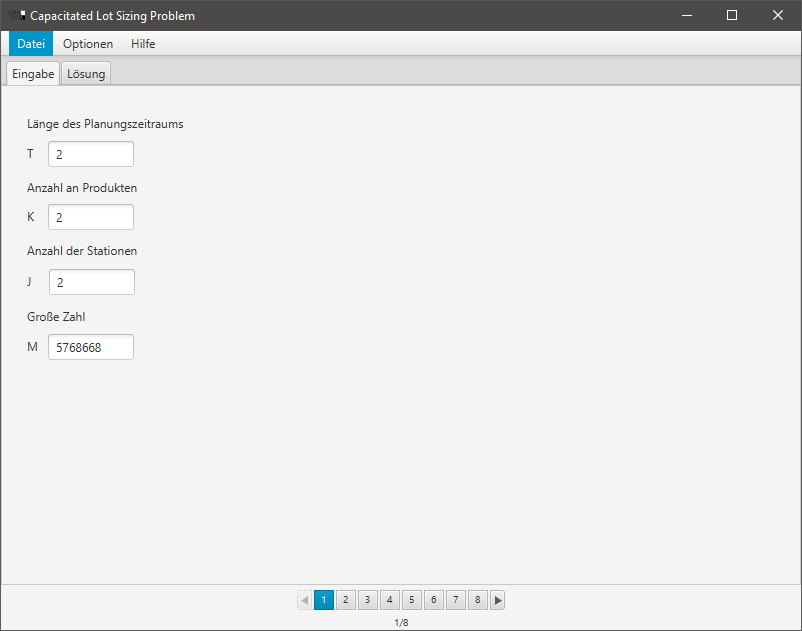
\includegraphics[width=1.0\linewidth]{images/CLSP_GUI.png} 
	\caption{Oberfläche des CLSP-Tools}
	\label{fig:clspgui}
\end{figure}

\subsection{Algorithmuseinstellung}
Unter dem Menüpunkt Optionen\textbackslash Algorithmuseinstellung kann festgelegt werden, ob das Modell mit Ganzzahlen oder Kommazahlen gespeichert und an ILOG übergeben wird.

\subsection{Manuelle Eingabe der Daten}

\paragraph{Eingabe - Seite 1}
Auf der ersten Seite werden 4 Eingabefelder angezeigt. Die Seite ist auch in Abbildung \ref{fig:clspgui} zu sehen. Diese müssen mit nachfolgenden Parametern gefüllt werden.

\begin{itemize}
	\item[T:] Länge des Planungszeitraums
	\item[K:] Anzahl an Produkten
	\item[J:] Anzahl der Stationen
	\item[M:] Große Zahl
\end{itemize}

Sind beim Verlassen der Seite keine Werte eingetragen, wird nachfolgende Fehlermeldung angezeigt.

\begin{figure}[H]
	\centering
	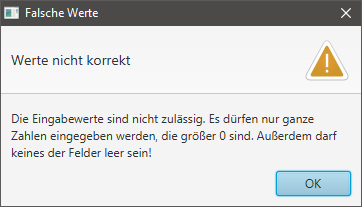
\includegraphics[width=.5\linewidth]{images/falscheWerte.png} 
	\caption{Anzeige bei falschen / fehlenden Werten}
	\label{fig:falscheWerte}
\end{figure}

Nach Bestätigung des Dialogs mit "'OK"' werden die vorhandenen Felder T, K und J mit "'1"' belegt. Große Zahl wird auf "'0"' festgelegt und muss händisch angepasst werden.

\paragraph{Eingabe - Seite 2}
Auf Seite 2 des Tabs "'Eingabe"' wird eine Matrix angezeigt die abhängig von den auf Seite 1 angegebenen Parametern T und K groß ist. Es wird die Nettobedarfsmenge je Produkt k in Zeitraum t in die Matrix eingetragen.

\begin{figure}[H]
	\centering
	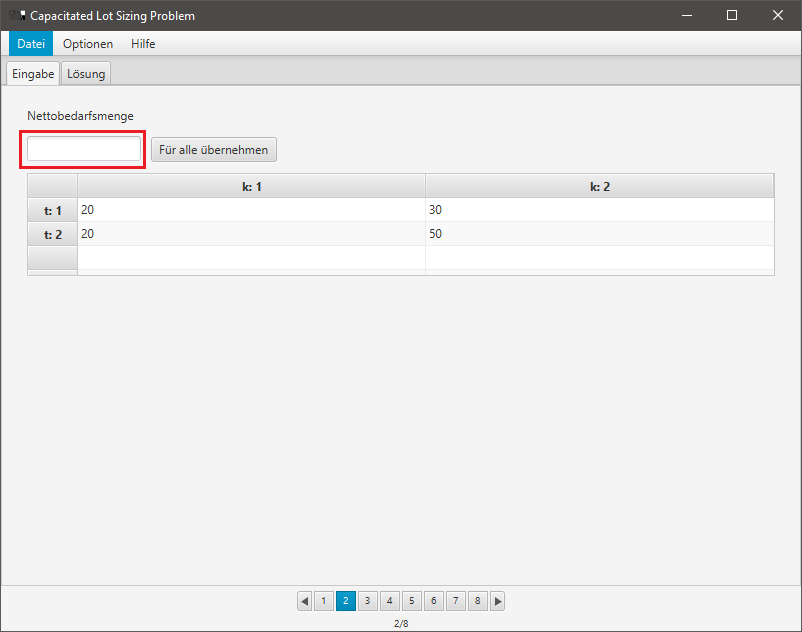
\includegraphics[width=.8\linewidth]{images/seite2.png} 
	\caption{Seite 2 - Nettobedarfsmenge}
	\label{fig:seite2}
\end{figure}

Es besteht die Möglichkeit jeden Wert der Matrix mit dem gleichen Wert zu belegen. Dazu wird die Zahl in das in Abbildung \ref{fig:seite2} rot markierte Eingabefeld eingetragen und durch den Button "'Für alle übernehmen"' übernommen.

\paragraph{Eingabe - Seite 3}
Seite 3 bietet die Möglichkeit die Parameter Lagerkostensätze, Rüstkostensätze und Mindestvorlaufzeiten je Produkt k festzulegen.

\begin{figure}[H]
	\centering
	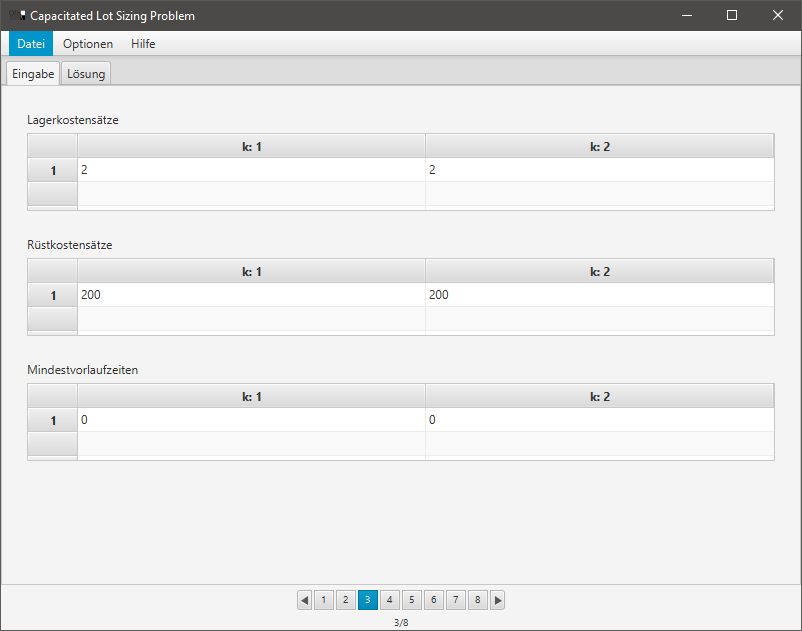
\includegraphics[width=.8\linewidth]{images/seite3.png} 
	\caption{Seite 3 - Lagerkostensätze, Rüstkostensätze und Mindestvorlaufzeiten}
	\label{fig:seite3}
\end{figure}

\pagebreak

\paragraph{Eingabe - Seite 4}
Anfangslagerbestand und Endlagerbestand werden auf Seite 4 für jedes Produkt k angegeben.

\begin{figure}[H]
	\centering
	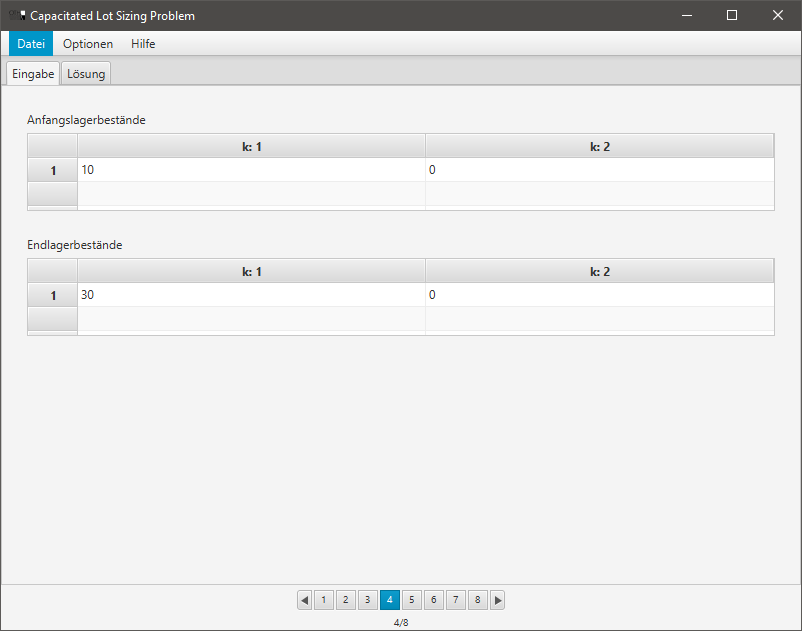
\includegraphics[width=.8\linewidth]{images/seite4.png} 
	\caption{Seite 4 - Anfangslagerbestand und Endlagerbestände}
	\label{fig:seite4}
\end{figure}

\pagebreak

\paragraph{Eingabe - Seite 5}
Seite 5 bietet die Eingabe für die Stückbearbeitungszeiten eines Produkts k je Station j. Wie auf Seite 1 kann ein Wert für alle Felder der Matrix mit Hilfe des Buttons "'Für alle übernehmen"' übernommen werden.

\begin{figure}[H]
	\centering
	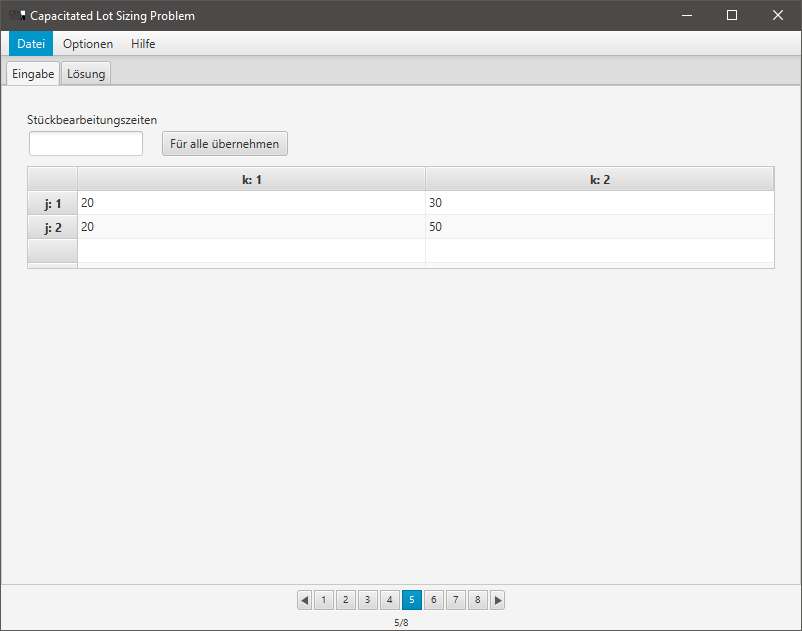
\includegraphics[width=.8\linewidth]{images/seite5.png} 
	\caption{Seite 5 - Stückbearbeitungszeiten}
	\label{fig:seite5}
\end{figure}

\paragraph{Eingabe - Seite 6}
Die Rüstzeiten werden auf Seite 6 festgelegt. Dabei wird je Produkt k und Station j ein Wert eingetragen. Auch diese Seite bietet den "'Für alle übernehmen"'-Button.

\begin{figure}[H]
	\centering
	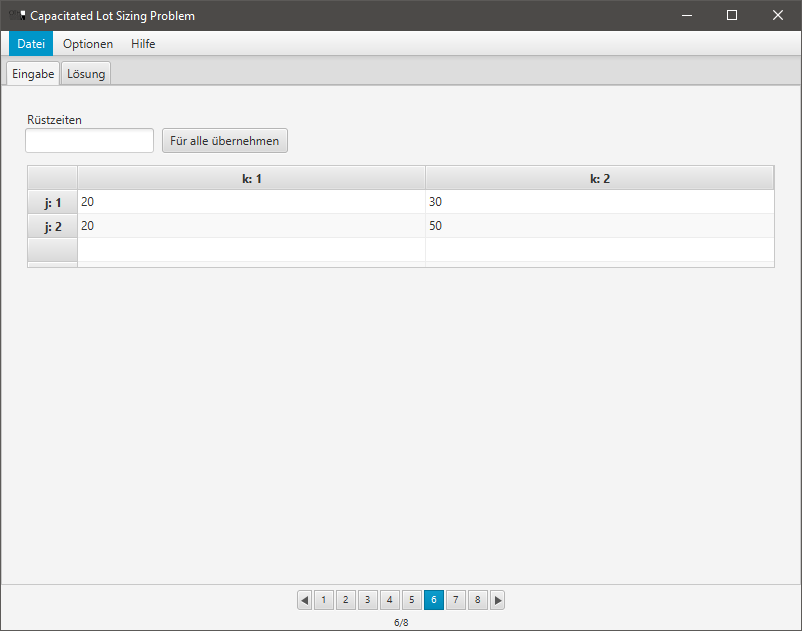
\includegraphics[width=.8\linewidth]{images/seite6.png} 
	\caption{Seite 6 - Maximale Zusatzkapazität}
	\label{fig:seite6}
\end{figure}

\paragraph{Eingabe - Seite 7}
Auf dieser Seite wird die verfügbare Kapazität je Station j und Planungszeitraum festgelegt. Es kann ebenfalls ein Wert für alle Felder der Matrix übernommen werden.

\begin{figure}[H]
	\centering
	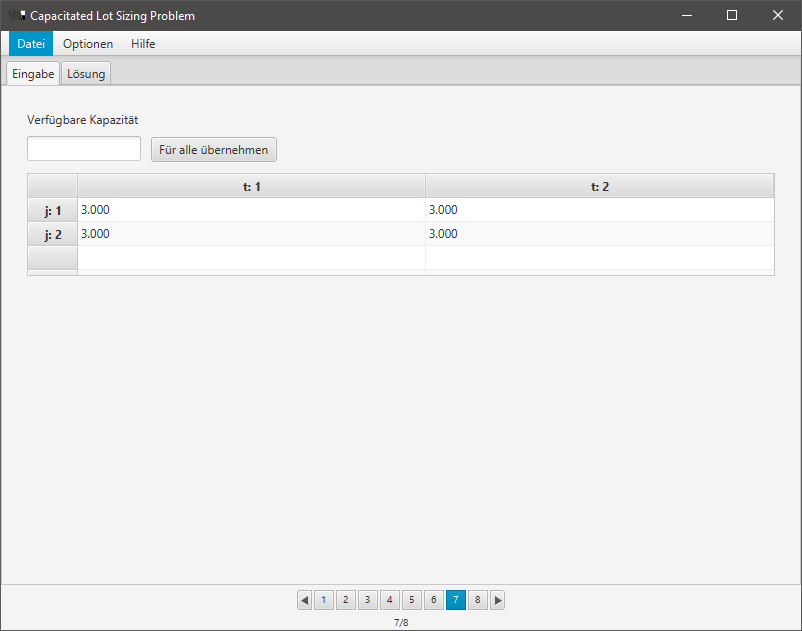
\includegraphics[width=.8\linewidth]{images/seite7.png} 
	\caption{Seite 7 - Verfügbare Kapazität}
	\label{fig:seite7}
\end{figure}

\pagebreak

\paragraph{Eingabe - Seite 8}
Seite 8 erlaubt die Festlegung des ILOG Parameters EPGAP ("'Relative Optimalitätslücke"'). Mit Hilfe des Buttons "'Berechnung starten"' kann die Berechnung durch ILOG angestoßen werden.

\begin{figure}[H]
	\centering
	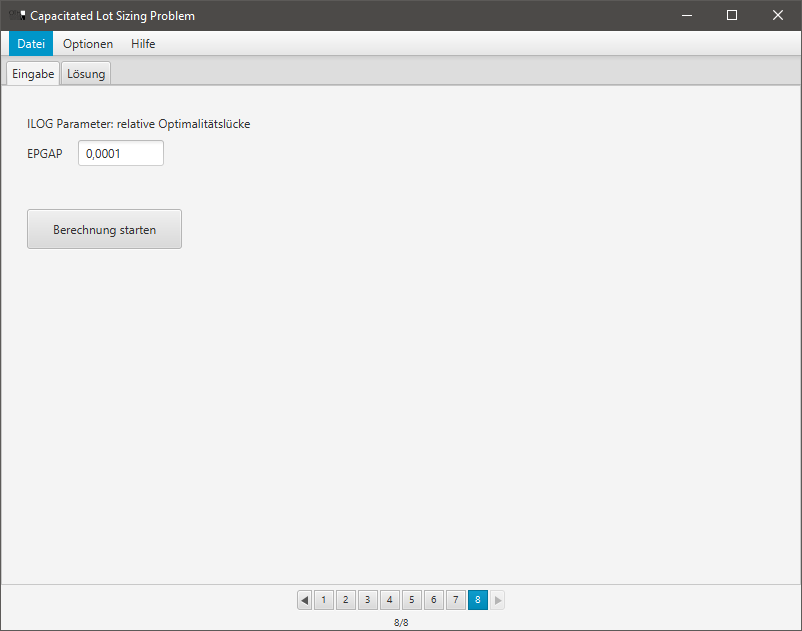
\includegraphics[width=.8\linewidth]{images/seite8.png} 
	\caption{Seite 8 - Relative Optimalitätslücke}
	\label{fig:seite8}
\end{figure}


\subsection{Funktionen des Dateimenüs}
Nachfolgend werden die Funktionen des Menüpunktes "'Datei"' beschrieben. Diese umfassen

\begin{itemize}
	\item Öffnen (Strg + O)
	\item Speichern (Strg + S)
	\item Berechnen (Strg + B)
	\item Stapelverarbeitung
	\item Schließen
\end{itemize}

Ist ein Shortcut angegeben kann dieser ebenfalls verwendet werden, um die Funktion aufzurufen.

\subsubsection{Speichern von DAT-Dateien}
Der Menüpunkt "'Speichern"' ruft einen Dialog auf. In diesem kann der gewünschte Speicherort und Dateiname angegeben werden. Dabei werden alle bereits gefüllten Werte in eine .dat-Datei geschrieben, um die Werte für eine spätere Verwendung wieder laden zu können.

\subsubsection{Öffnen von DAT-Dateien}
Es ist möglich zuvor gespeicherte .dat-Dateien wieder zu laden. Der Punkt Datei\textbackslash Öffnen öffnet einen Dialog, in dem die zu ladende Datei ausgewählt werden kann.

\subsubsection{Berechnung starten}
Die Berechnung kann (wie auf Seite 8) ebenfalls mit Hilfe dieses Menüpunkts angestoßen werden.

\subsubsection{Stapelverarbeitung}
Der Menüpunkt "'Stapelverarbeitung"' öffnet den nachfolgenden Dialog.

\begin{figure}[H]
	\centering
	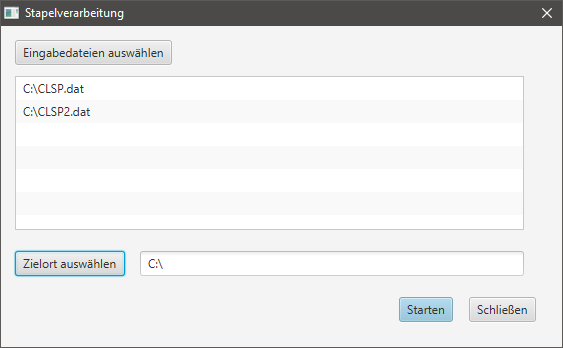
\includegraphics[width=.7\linewidth]{images/stapelverarbeitung.png} 
	\caption{Dialog Stapelverarbeitung}
	\label{fig:stapel}
\end{figure}

Der Button "'Eingabedateien auswählen"' öffnet einen weiteren Dialog, in dem mehrere .dat-Dateien gewählt werden können. Die Dateinamen werden anschließend in der Liste angezeigt. Mit Hilfe des Buttons "'Zielort auswählen"' kann der Ordner ausgewählt werden, in dem die Dateien mit der Lösung abgelegt werden.

\subsection{Anzeige der Lösung}
Der Tab "'Lösung"' zeigt nach der erfolgreichen Berechnung des Problems das Ergebnis an. Nachfolgende Abbildung zeigt dabei den Tab mit dem Ergebnis für die in der .zip-Datei beinhaltete und in diesem Handbuch verwendeten Testdatei.

\begin{figure}[H]
	\centering
	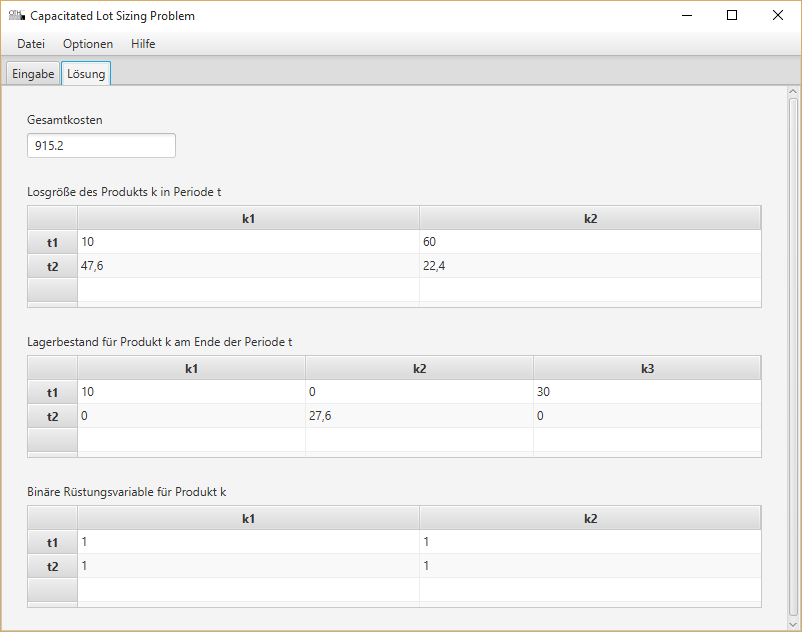
\includegraphics[width=1.0\linewidth]{images/loesung.png} 
	\caption{Tab - Lösung}
	\label{fig:loesung}
\end{figure}

\pagebreak

%-------------------------------------------------------------------------------------
% Verzeichnisse %-------------------------------------------------------------------------------------
%	\rhead{Verzeichnisse} %Kopftextbeschriftung
%
%	\stepcounter{section}
%	\phantomsection \label{Verzeichnisse}
%	\addcontentsline{toc}{section}{Verzeichnisse} %Ohne Nummer ins Inhaltsverzeichnis
%	\renewcommand{\thesection}{\Roman{verzeichnis}}
%	\section*{Verzeichnisse}
%	% Literaturverzeichnis
%	\rhead{Verzeichnisse}
%	\renewcommand{\refname}{Literaturverzeichnis}
%	\printbibliography
%	\pagebreak
	
	% Abbildungsverzeichnis
	%\stepcounter{verzeichnis}
	\listoffigures
	\pagebreak
	
	% Tabellenverzeichnis
%	\stepcounter{verzeichnis}
%	\listoftables
%	\pagebreak
	
	% Abkürzungen
%	\stepcounter{verzeichnis}
	\section{Abkürzungsverzeichnis}
	\vspace{-6em} % Abstand analog der anderen Verzeichnisse reduzieren
	\printnoidxglossary[type=\acronymtype,style=alttree,title=,toctitle=] %automatischen Titel und Gliederungsbeschriftung unterdrücken - sonst steht da Glossarie
	%\newpage

\end{document}
